\chapter{Wst�p}
\section{Cel projektu}
Celem niniejszej pracy by�o stworzenie aplikacji webowej, wspomagaj�cej kontakt pomi�dzy lekarzem, a pacjentem. Docelowo, aplikacja powinna umo�liwia� wymian� danych na bie��co. Pacjent powinien mie� mo�liwo�� rozpocz�cia rozmowy z wszystkimi lekarzami dost�pnymi on--line. Za�o�ono, i� aplikacja stanowi narz�dzie, wspomagaj�ce istniej�c� ju� przychodni� lekarsk�.

Osi�gni�cie celu wymaga�o realizacji nast�puj�cych etap�w:
\begin{itemize}
\item przydzia�u zada� poszczeg�lnym osobom w grupie
\item wyboru narz�dzi
\item opracowania architektury bazy danych
\item stworzenia interfejsu u�ytkownika
\item implementacji poszczeg�lnych funkcjonalno�ci
\end{itemize}
\section{Platforma projektowa}
\section{Harmonogram prac}
\section{Przegl�d rynku}

\chapter{System}
\section{Architektura systemu}
\section{Funkcje wewn�trzne}
\section{Przypadki testowe}

\chapter{Wnioski}

%\begin{figure}[!htb]
%	\centering
%	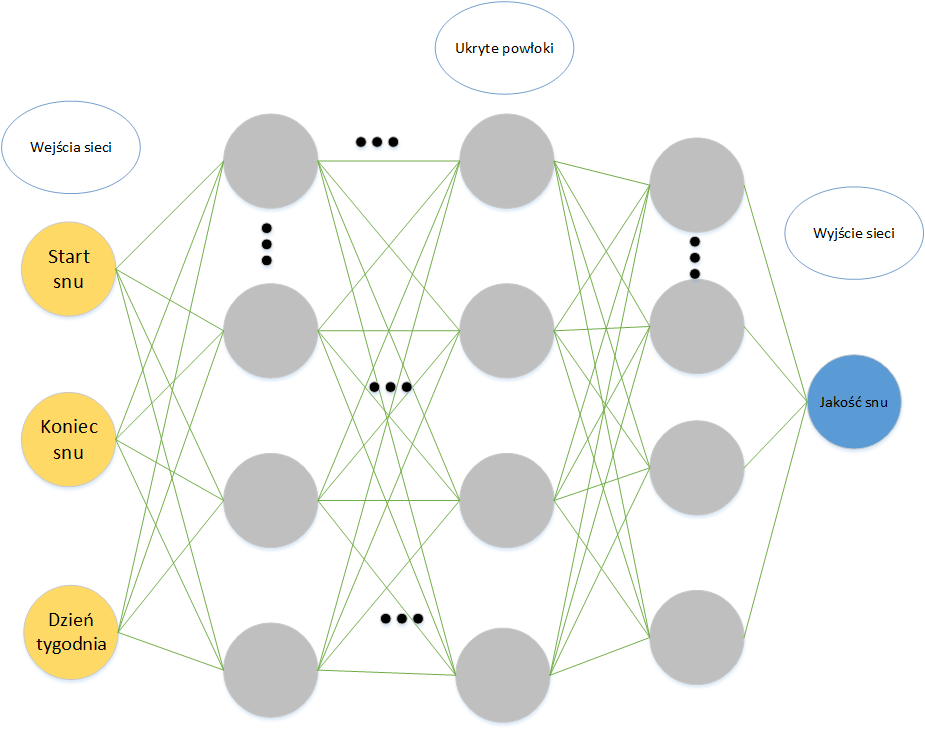
\includegraphics[width=1\textwidth]{lstm_schema}
%	\caption{Zaprojektowana sie� neuronowa.}\label{lstm-schema}
%\end{figure}



